\chapter{Process Mining}

\section{Software Process Recovery}
Software development process was always being under focus of various stakeholders due to the number of reasons ranging from standards compliance to business and security intelligence. When no live observations are made on the performers, due to the availability, timing, cost, or privacy issues, recovering software process from artifacts could be complex and expensive process. Researchers have suggested a possibility of software process recovery by interviewing of developers and managers and by analysis of process artifacts: such as printed documents - designs, use-cases, software inspections or electronic artifact trails: version, bug and issue control systems and mailing lists. This research resulted in many published work:
\begin{itemize}
\item{Cook \& Wolf in \cite{citeulike:328044} discuss an event-based framework for process discovery based on grammar inference and finite state machines. The authors directly applied their framework to Software Configuration Management (SCM) logs demonstrating satisfactory results.}
\item{Jensen \& Scacchi \cite{citeulike:5043664} describe an interesting framework built upon mapping between process artifacts and process entities into an universal generic meta-model. Application of their human-involved technique leveraged a pre-existing domain knowledge for the effective pruning and iterative process revision resulted in ``workflows discovery''.}
\item{German in \cite{citeulike:421438} performed a manual mining of the GNOME process artifacts: documentations, CVS logs, and one hundred and four mailing-lists in order to
describe the development processes from GSD (Global Software Development) point of view.}
\item{Ripoche tried a more automatic approach in \cite{citeulike:9112798} by developing a generic model for process-based explanation of bugs persistence using state diagrams and
probabilistic choices.}
\end{itemize}
All these suggests that software process artifacts bear enough information about performed process for its recontsruction. In my study I havily relying on this fact. This not only serves as a foundation of my hypothesis, but also partially assures the validity of my approach to the software process reconstruction. Further in this chapter I will introduce a novel technique of pattern mining form the software process artifacts trails. After introduction of the technique, I will walk through the performed case studies in which I have applied this technique to the various types of the software process artifact trails.

\subsection{Apriori algorithm}

Family of seminal Apriori algorithms was proposed in 1994 by Agrawal \& Srikant \cite{citeulike:775528}. These algorithms are based on the naive \textit{apriori association rule} stating that \textit{any sub-pattern of a frequent pattern must be frequent}. The name ``apriori'' is based on the fact of using of a prior knowledge by the algorithm: the $k$-th itemsets are used to generate $(k+1)$ itemsets.

Algorithm starts by scanning a database and finding all possible $1$-itemsets counting their support and keeping only those which satisfy to the minimal support value. This itemsets result in the set $L_{1}$. This set, in turn, is used to construct $L_{2}$ set which is a combination of all possible itemsets from $L_{1}$, once construction of $L_{2}$ complete one full scan of the database required to compute the support of each of the itemsets. For finding the $L_{3}$ and so on the Apriori property is used, which reduces the search space while generating candidates. Apriori property is that \textit{all non-empty subsets of the frequent itemset must be also frequent}.

The apriori property is used in the candidate itemset generation step in the next fashion: if itemset $I$ does not satisfies to minimal support value, i.e. $Support(I) \; \leq \; min\_support$, the itemset $I'$ resulting from adding item $i$ into the $I$ ($I' = I \cup i$) cannot occur mor efrequently than $I$, i.e. $Support(I') \; \leq \; min\_support$. In some literature this property called \textit{antimonotone} property as an opposite to monotone one.

The generation of itemsets $L_{k}$ for $k > 2$ consists of two steps: join and prune.

\textbf{The Join step.}

To find itemset $L_{k}$ based on $L_{k-1}$ we first generate the set $C_{k}$ - the set of all candidate patterns based on the join of $L_{k-1}$ with itself: $L_{k-1} \times L_{k-1}$. We will introduce a notation $l_{i,j}$ for $j$th item of the itemset $i$, also we must note, that by convention, Apriori assumes that all items within an itemset $l_{i}$ are sorted alphabetically, i.e. that $l_{i,j} < l_{i,j+1}$. Taking all above in the account, the join of $L_{k-1} \times L_{k-1}$ is performed only on itemsets $l_{i}$ and $l_{j}$ if their first $k-2$ items are the same, i.e. $l_{i,m} = l_{j,m}, \; \forall m \in [0,k-2]$, this generates next candidate itemsets: ${l_{i,1},l_{i,2},l_{i,3},...,l_{i,k-1},l_{j,k-1}}$. Here we are also making sure that $l_{i,k-1} < l_{j,k-1}$ to avoid duplicates within $C_{k}$.

\textbf{The Prune step.}

The set $C_{k}$ generated during the join step is a superset of $L_{k}$ and it's members may not be frequent enough to satisfy a minimal support value.


\section{Symbolic Aggregate approXimation (SAX)} \label{sax}
\begin{figure}[tbp]
   \centering
   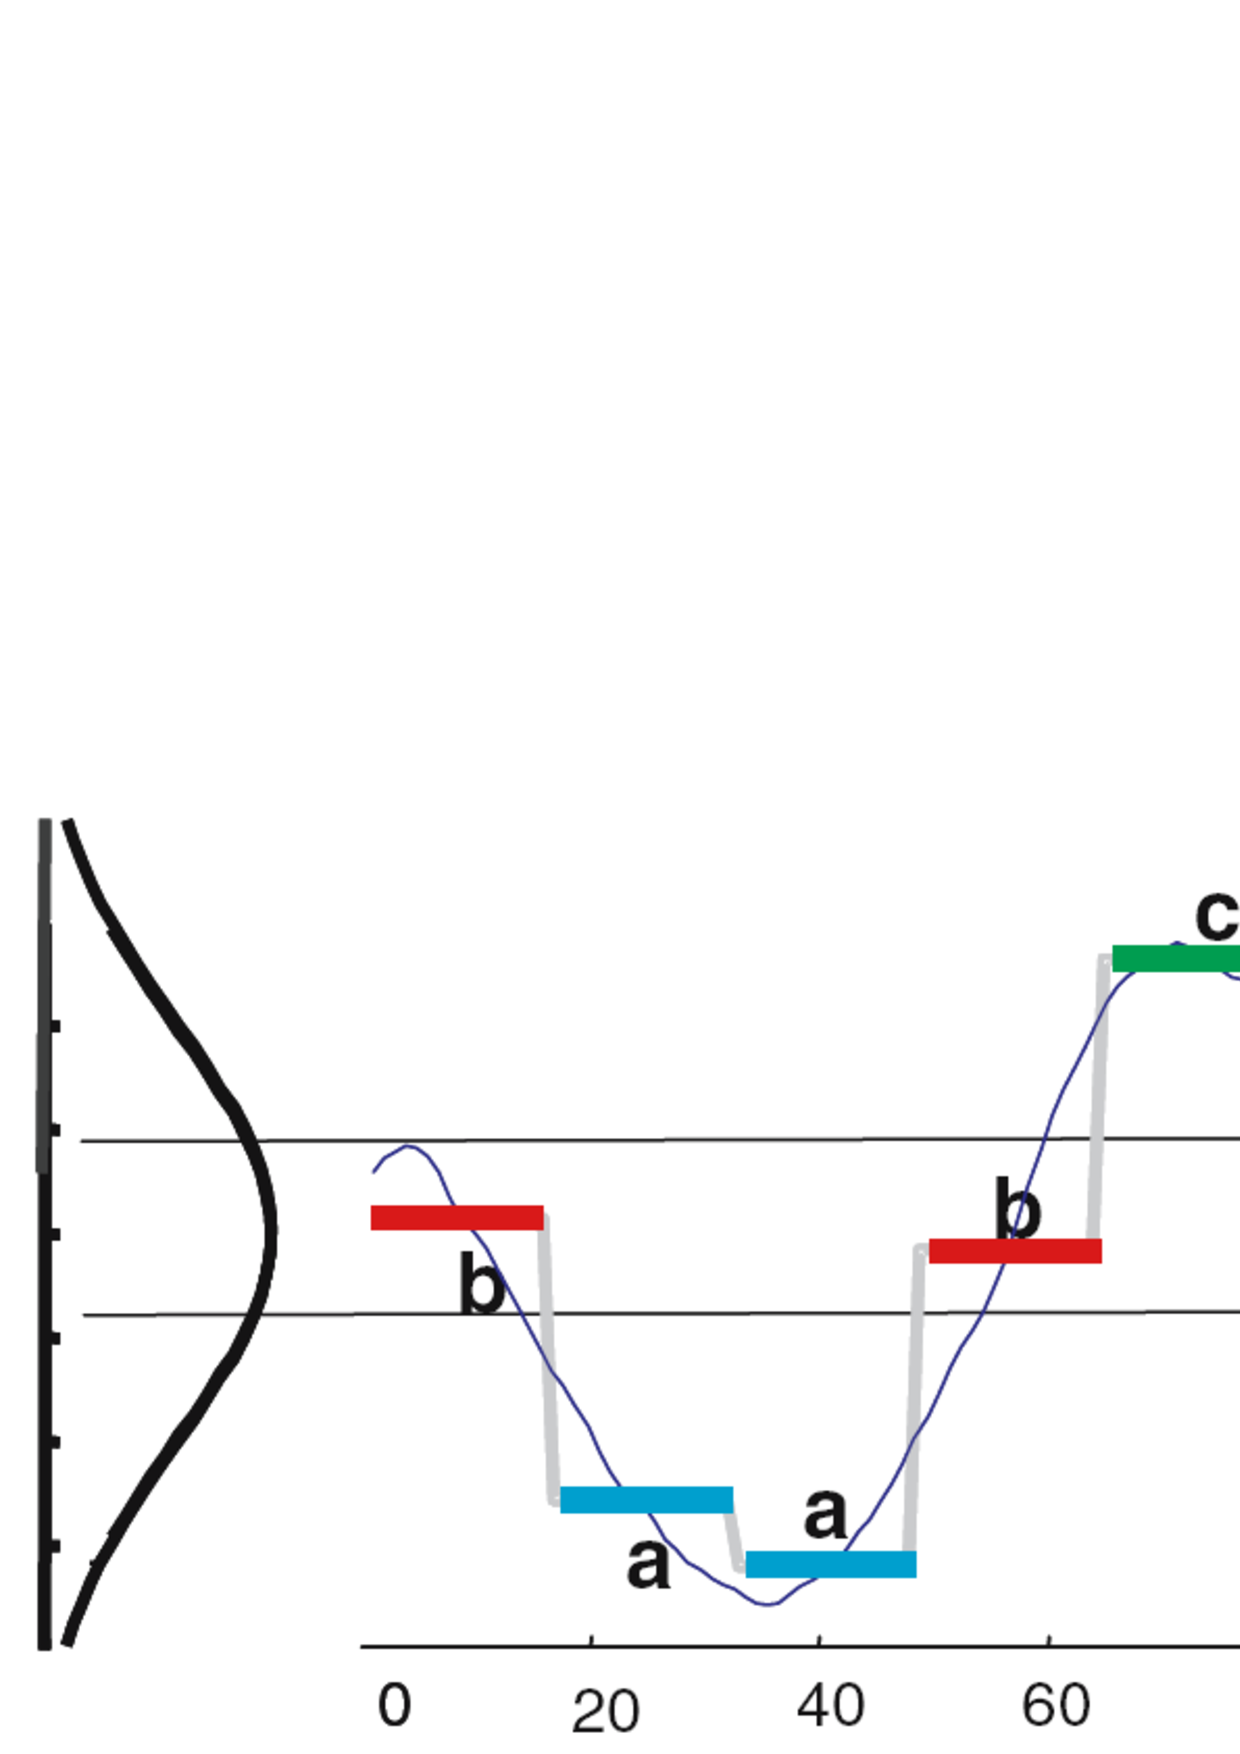
\includegraphics[height=45mm]{sax_intro}
   \caption{The illustration of the SAX approach taken from \cite{citeulike:2821475} depicts two pre-determined breakpoints for the three-symbols alphabet and the conversion of the time-series of length $n=128$ into PAA representation followed by mapping of the PAA coefficients into SAX symbols with $w=8$ and $a=3$ resulting in the string \textbf{baabccbc}.}
   \label{fig:sax_intro}
\end{figure}

Symbolic Aggregate approXimation was proposed by Lin et al. in \cite{citeulike:2821475}. This method extends the PAA-based approach \cite{citeulike:2946589} \cite{citeulike:3000416}, inheriting algorithmic simplicity and low computational complexity, while providing satisfiable sensitivity and selectivity in range-query processing. Moreover, the use of a symbolic representation opens the door to the existing wealth of data-structures and string-manipulation algorithms in computer science such as hashing, regular expression pattern matching, suffix trees etc.

SAX transforms a time-series $X$ of length $n$ into a string of arbitrary length $\omega$, where $\omega << n$ typically, using an alphabet $A$ of size $ a \geq 2$. The SAX algorithm consist of two steps: during the first step it transforms the original time-series into a PAA representation and this intermediate representation gets converted into a string during the second step. Use of PAA at the first step brings the advantage of a simple and efficient dimensionality reduction while providing the important lower bounding property as shown in the previous section. The second step, actual conversion of PAA coefficients into letters, is also computationally efficient and the contractive property of symbolic distance was proven by Lin et al. in \cite{citeulike:532335}.

\begin{equation}
D_{PAA}(\bar{X}, \bar{Y}) \equiv \sqrt{\frac{n}{M}} \sqrt{ \sum_{i=1}^{M} 
\left(  \bar{x}_{i} - \bar{y}_{i} \right)}
\label{eq:paa_distance}
\end{equation}

Discretization of the PAA representation of a time-series into SAX is implemented in a way which produces symbols corresponding to the time-series features with equal probability. The extensive and rigorous analysis of various time-series datasets available to the authors has shown that normalized by the zero mean and unit of energy time-series follow the Normal distribution law. By using Gaussian distribution properties, it's easy to pick $a$ equal-sized areas under the Normal curve using  lookup tables  \cite{citeulike:4434481} for the cut lines coordinates, slicing the under-the-Gaussian-curve area. 
The $x$ coordinates of these lines called ``breakpoints'' in the SAX algorithm context. The list of breakpoints $B=\beta_{1}, \beta_{2}, ... , \beta_{a-1}$ such that $\beta_{i-1} < \beta_{i}$ and $\beta_{0} = -\infty$, $\beta_{a} = \infty$ divides the area under $N(0,1)$ into $a$ equal areas. By assigning a corresponding alphabet symbol $alpha_{j}$ to each interval $[\beta_{j-1},\beta_{j})$, the conversion of the vector of PAA coefficients $\bar{C}$ into the string $\hat{C}$ implemented as follows:
\begin{equation}
\hat{c}_{i} = alpha_{j}, \; \text{iif} \; \bar{c}_{i} \in [\beta_{j-1},\beta_{j})
\label{eq:alpha}
\end{equation}

\begin{figure}[tbp]
   \centering
   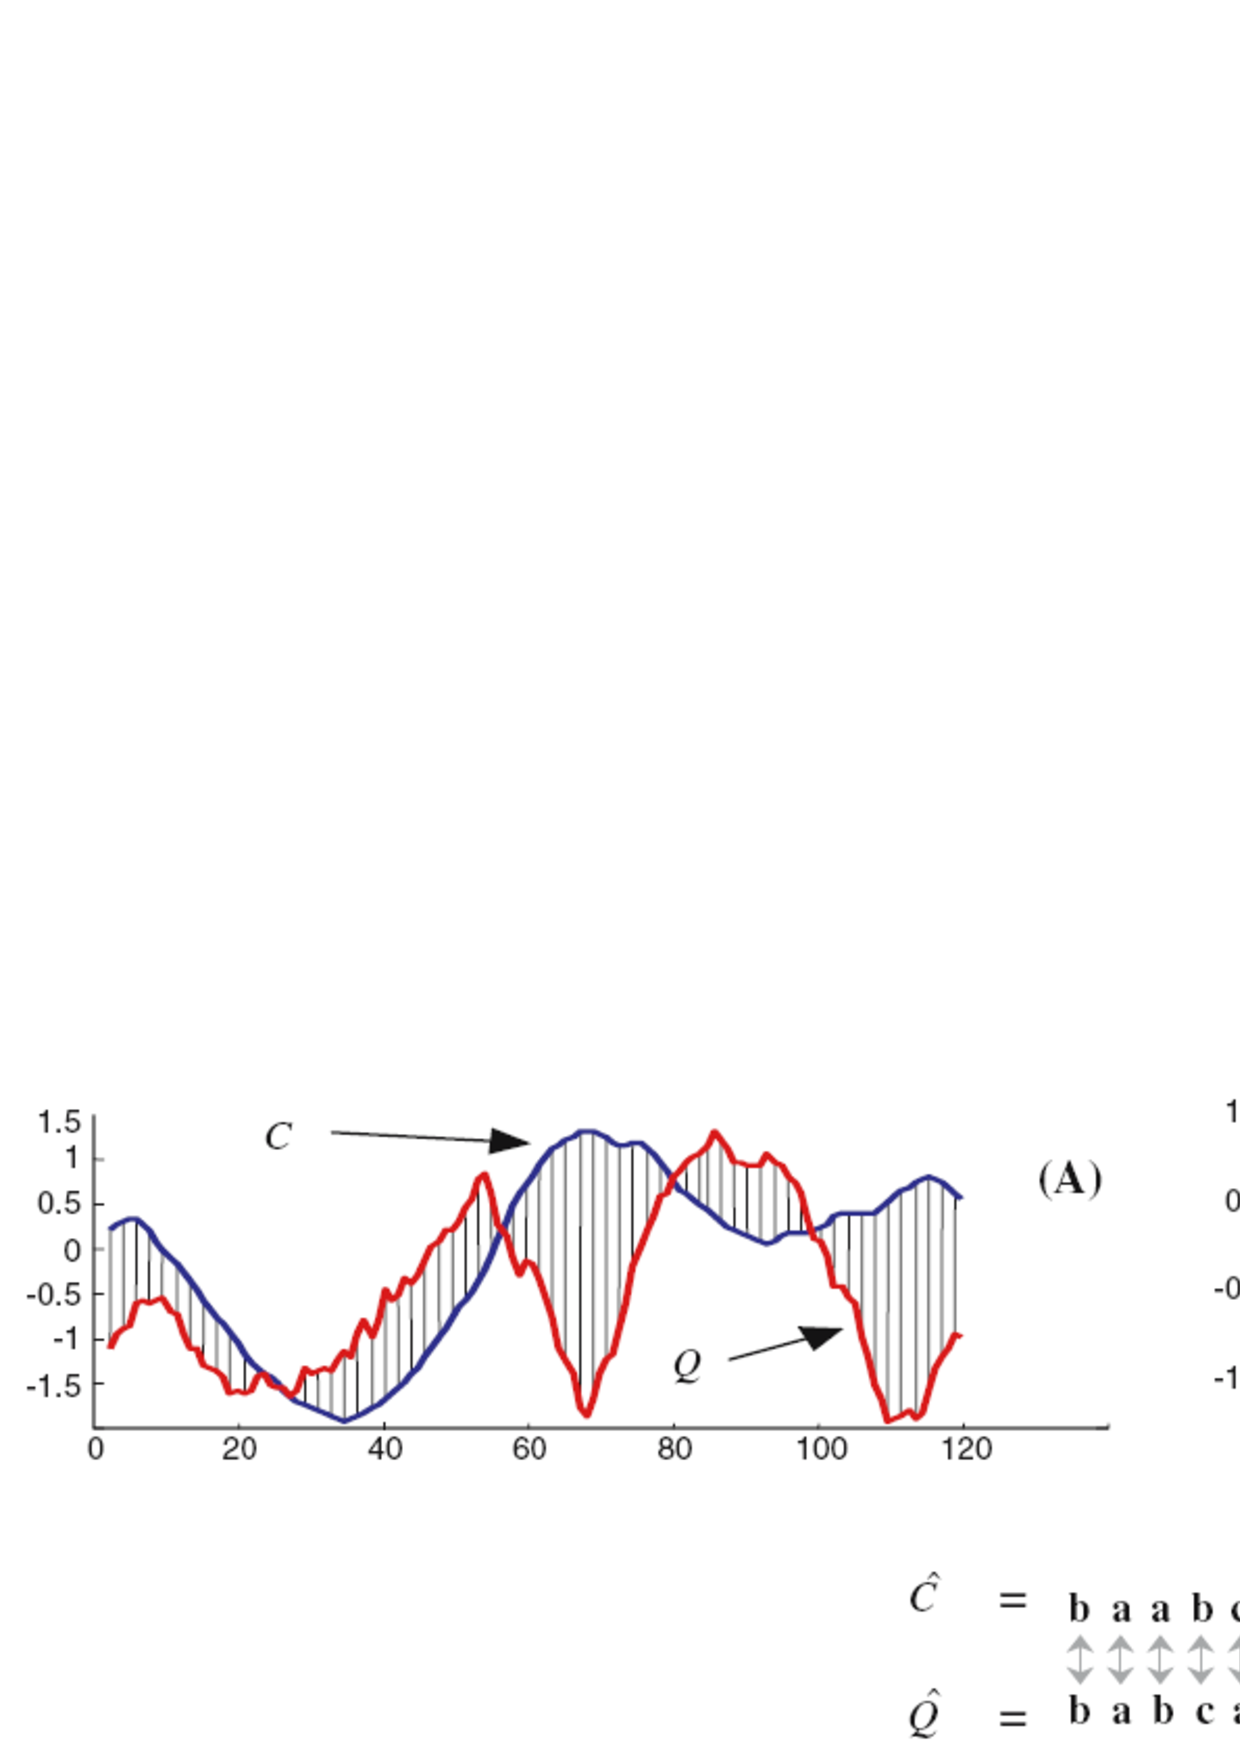
\includegraphics[height=47mm]{sax_distance}
   \caption{The visual representation of the two time-series $Q$ and $C$ and three distances between their representation: Euclidean distance between raw time-series (A), the distance defined for PAA coefficients (B) and the distance between two SAX representations (C). (The figure taken from \cite{citeulike:2821475} as well)}
   \label{fig:sax_distance}
\end{figure}

SAX introduces new metrics for measuring distance between strings by extending Euclidean and PAA (\ref{eq:paa_distance}) distances. The function returning the minimal distance between two string representations of original time series $\hat{Q}$ and $\hat{C}$ is defined as
\begin{equation}
MINDIST(\hat{Q},\hat{C}) \equiv \sqrt{ \frac{n}{w} } \sqrt{ \sum_{i=1}^{w} ( dist( \hat{q}_{i}, \hat{c}_{i} ) )^{2}}
\label{eq:sax_mindist}
\end{equation} 
where the $dist$ function is implemented by using the lookup table for the particular set of the breakpoints (alphabet size) as shown in Table \ref{tbl:sax_lookup}, and where the singular value for each cell $(r,c)$ is computed as 
\begin{equation}
cell_{(r,c)} = 
\begin{cases} 
0, \text{ if }\left| r-c \right| \leq 1 \\
\beta_{\max(r,c) - 1} - \beta_{\min(r,c) - 1}, \text{ otherwise}
\end{cases}
\label{eq:cell}
\end{equation}

\begin{table}
\begin{tabularx}{400pt}{X X X X X}
\hline
   & a   & b    & c    & d    \\
\hline
a & 0    & 0    & 0.67 & 1.34 \\
b & 0    & 0    & 0    & 0.67 \\
c & 0.67 & 0    & 0    & 0    \\
d & 1.34 & 0.67 & 0    & 0    \\
\hline
\end{tabularx}
\caption{A lookup table used by the MINDIST function for the $a=4$}
\label{tbl:sax_lookup}
\end{table}

As shown by Li et al., this SAX distance metrics lower-bounds the PAA distance, i.e.
\begin{equation}
\sum_{i=1}^{n} (q_{i} - c_{i})^{2} \geq n(\bar{Q} - \bar{C})^{2} \geq n(dist(\hat{Q},\hat{C}))^2
\label{eq:sax_bounding}
\end{equation}

The SAX lower bound was examined by Ding et al. \cite{citeulike:4501572} in great detail and found to be superior in precision to the spectral decomposition methods on bursty (non-periodic) data sets.


